\begin{figure}[htbp]
			\centering
			\resizebox{\textwidth}{!}{%
				\begin{tikzpicture}[scale=0.95,>=latex,
					trave/.style={line width=1.4pt},
					carico/.style={black, line width=0.6pt},
					forza/.style={black, line width=0.8pt},
					diagT/.style={black, line width=0.7pt},
					diagM/.style={black, line width=0.7pt},
					hatch/.style={gray!50, line width=0.3pt},
					rif/.style={densely dashed, black, line width=0.5pt},
					quota/.style={black, line width=0.4pt},
					]
					\def\tw{0.15}\def\thR{0.28}\def\rn{0.06}
					\def\rw{0.05}\def\bw{0.09}\def\gw{0.22}\def\hh{0.10}
					\def\Lell{4}\pgfmathsetmacro{\xMid}{0.5*\Lell}
					\def\pBot{0.45}\def\pTop{0.95}
					\def\rCoppia{0.24}\def\Lwing{0.12}\def\AoffX{0.20}\def\BoffX{0.20}
					\def\ylab{-1.55}
					\def\cerniera#1{%
						\draw[thick] (#1,0) -- (#1-\tw,-\thR) -- (#1+\tw,-\thR) -- cycle;
						\draw[thick] (#1-\gw,-\thR) -- (#1+\gw,-\thR);
						\foreach \x in {-0.16,-0.08,0,0.08,0.16}\draw[thin] (#1+\x,-\thR) -- ++(-0.07,-\hh);
						\draw[thick, fill=white] (#1,0) circle (\rn);}
					\def\carrello#1{%
						\draw[thick] (#1,0) -- (#1-\tw,-\thR) -- (#1+\tw,-\thR) -- cycle;
						\draw[thick] (#1-\bw,-\thR-\rw-0.01) circle (\rw);
						\draw[thick] (#1+\bw,-\thR-\rw-0.01) circle (\rw);
						\draw[thick] (#1-\gw,-\thR-2*\rw-0.04) -- (#1+\gw,-\thR-2*\rw-0.04);
						\foreach \x in {-0.16,-0.08,0,0.08,0.16}\draw[thin] (#1+\x,-\thR-2*\rw-0.04) -- ++(-0.07,-\hh);
						\draw[thick, fill=white] (#1,0) circle (\rn);}
					\def\caricodist{%
						\draw[carico] (0,\pBot) rectangle (\Lell,\pTop);
						\foreach \x in {0,0.8,1.6,2.4,3.2,4.0}\draw[->, carico] (\x,\pTop) -- (\x,\pBot);
						\node[right, font=\small] at (\Lell+0.06,{0.5*(\pBot+\pTop)}) {$\bar{p}$};}
					\def\coppiaA#1{%
						\draw[forza] (\AoffX,-\rCoppia) arc[start angle=-90, end angle=90, radius=\rCoppia];
						\draw[forza] (\AoffX,\rCoppia) -- ({\AoffX+\Lwing*cos(25)},{\rCoppia+\Lwing*sin(25)});
						\draw[forza] (\AoffX,\rCoppia) -- ({\AoffX+\Lwing*cos(-25)},{\rCoppia+\Lwing*sin(-25)});
						\node[font=\footnotesize] at (\AoffX+0.28,\rCoppia+0.06) {#1};}
					\def\coppiaB#1{%
						\draw[forza] (\Lell-\BoffX,\rCoppia) arc[start angle=90, end angle=270, radius=\rCoppia];
						\draw[forza] (\Lell-\BoffX,-\rCoppia) -- ({\Lell-\BoffX+\Lwing*cos(155)},{-\rCoppia+\Lwing*sin(155)});
						\draw[forza] (\Lell-\BoffX,-\rCoppia) -- ({\Lell-\BoffX+\Lwing*cos(205)},{-\rCoppia+\Lwing*sin(205)});
						\node[font=\footnotesize] at (\Lell-\BoffX-\rCoppia-0.10,-0.30) {#1};}
					
					% ===== (a) sistema principale =====
					\begin{scope}[xshift=0cm]
						\draw[trave] (0,0) -- (\Lell,0);
						\cerniera{0}\carrello{\Lell}
						\caricodist
						\coppiaA{$\chi_1$}\coppiaB{$\chi_2$}
						\node[above left, font=\small] at (0,0.04) {$A$};
						\node[above right=-1pt, font=\small] at (\Lell,0.04) {$B$};
						\node[font=\small] at (\xMid/2,\ylab/2) {(a)};
					\end{scope}
					% ===== (b) T = T_0 + (chi1+chi2)/l =====
					\begin{scope}[xshift=6.0cm]
						\def\kT{2.0}                              % zoom del pannello taglio
						\pgfmathsetmacro{\hT}{0.42*\kT}           % p l /2
						\pgfmathsetmacro{\cT}{\hT/3}              % (chi1+chi2)/l = (1/3)(p l /2)  [chi=p l^2/12]
						\draw[trave] (0,0) -- (\Lell,0);
						\foreach \x in {0.1,0.3,...,3.9}{\pgfmathsetmacro{\h}{\cT+\hT*(1-2*\x/\Lell)}\draw[hatch] (\x,0)--(\x,\h);}
						\draw[diagT] (0,0)--(0,{\cT+\hT}) -- (\Lell,{\cT-\hT}) -- (\Lell,0);
						\draw[rif] (0,\cT)--(\Lell,\cT);
						\cerniera{0}\carrello{\Lell}
						\node[above left, font=\small] at (0,0.04) {$A$};
						\node[above right=-1pt, font=\small] at (\Lell,0.04) {$B$};
						\node[font=\footnotesize] at (0.5,0.55) {$\boldsymbol{\oplus}$};
						\node[font=\footnotesize] at (3.55,-0.18) {$\boldsymbol{\ominus}$};
						% trattini di richiamo ai valori estremi e alla costante
						\draw[quota, <-] (0,{0.55*(\cT+\hT)}) -- (0.55,{\cT+\hT+0.30});
						\node[right, font=\scriptsize] at (0.52,{\cT+\hT+0.30}) {$\tfrac{\bar p\ell}{2}+\tfrac{\chi_1+\chi_2}{\ell}$};
						\draw[quota, <-] (\Lell,{\cT-\hT/2}) -- (\Lell-1.0,{\cT-\hT/2-0.50});
						\node[below left=-3pt, font=\scriptsize] at (\Lell+0.16,{\cT-\hT-0.14}) {$-\tfrac{\bar p\ell}{2}+\tfrac{\chi_1+\chi_2}{\ell}$};
						\draw[quota, <-] (2.55,\cT) -- (2.55,{\cT+0.34});
						\node[above, font=\scriptsize] at (2.55,{\cT+0.32}) {$\tfrac{\chi_1+\chi_2}{\ell}$};
						\node[font=\small] at (\xMid/2,\ylab/2) {(b)};
					\end{scope}
					% ===== (c) M = M_0 + retta di chiusura =====
					\begin{scope}[xshift=12.0cm]
						\def\kM{1.5}                              % zoom del pannello momento
						\pgfmathsetmacro{\sag}{0.52*\kM}          % p l^2/8
						\pgfmathsetmacro{\mA}{2*\sag/3}           % chi_1 = (2/3)(p l^2/8)  [chi=p l^2/12]
						\pgfmathsetmacro{\mB}{2*\sag/3}           % chi_2
						\draw[trave] (0,0) -- (\Lell,0);
						\foreach \x in {0.1,0.3,...,3.9}{\pgfmathsetmacro{\u}{\x/\Lell}\pgfmathsetmacro{\h}{\mA-(\mA+\mB)*\u-\sag*4*\u*(1-\u)}\draw[hatch] (\x,0)--(\x,\h);}
						\draw[diagM] (0,0)--(0,\mA) plot[domain=0:\Lell,samples=90] (\x,{\mA-(\mA+\mB)*(\x/\Lell)-\sag*4*(\x/\Lell)*(1-\x/\Lell)}) -- (\Lell,0);
						\draw[rif] (0,\mA)--(\Lell,-\mB);
						\cerniera{0}\carrello{\Lell}
						\node[above left, font=\small] at (0,0.04) {$A$};
						\node[above right=-1pt, font=\small] at (\Lell,0.04) {$B$};
						\draw[<->, quota] (\xMid,{(\mA-\mB)/2})--(\xMid,{(\mA-\mB)/2-\sag});
						\node[right, font=\scriptsize] at (\xMid+0.05,{(\mA-\mB)/2-0.5*\sag}) {$\tfrac{\bar p\ell^2}{8}$};
						\node[above, font=\scriptsize] at (0,\mA+0.02) {$-\chi_1$};
						\node[right, font=\scriptsize] at (\Lell+0.06,-\mB-0.02) {$\chi_2$};
						\node[font=\small] at (\xMid/2,\ylab/2) {(c)};
					\end{scope}
				\end{tikzpicture}
			}
			\caption{Soluzione generale (sistema principale, a): taglio
				$T = T_0 + \chi_1 T_1 + \chi_2 T_2$ (b), retta $T_0$ traslata
				della costante $(\chi_1+\chi_2)/\ell$; momento
				$M = M_0 + \chi_1 M_1 + \chi_2 M_2$ (c), parabola $M_0$ appesa
				alla retta di chiusura da $-\chi_1$ in $A$ a $\chi_2$ in $B$.
				I diagrammi (b)--(c) sono tracciati per la scelta illustrativa
				$\chi_1 = \chi_2 = \bar p\,\ell^2/12$; i valori effettivi si
				ottengono imponendo la congruenza (Vol.~II).}
			\label{fig:stat_iper_trasv_01-s}
		\end{figure}
